%!TEX root = ../Main.tex

\chapter{Support vector machines}
In this chapter we’ll discuss the subject Support Vector Machines (SVM). SVM performs well in a variety of settings and are often considered one of the best “out of the box “classifiers.  In this chapter we’ll touch upon two different variants of SVM. First, the simple an intuitive classifier called maximal margin classifier, which the support vector machine is a generalization of. Although the \textit{Maximal Margin Classifier} is elegant and simple, there is a lot of datasets where the classifier can’t be applied, because it requires the classes to be separated by a linear boundary. So, we’ll also touch upon an extension of the \textit{Maximal Margin Classifier} called the \textit{Support Vector Classifier}, which can be applied to a broader range of datasets. 

\section{Maximal Margin Classifier}
Maximal Margin Classifier is the simplest of different type of SVM. It tries to find a plane that separates the classes in the feature space. When we talk about a plane to separate the classes, we talk about a hyperplane. 

A hyperplane in \textit{p} dimensions is a flat affine subspace of dimensions \textit{p}-1. If we’ll look at two dimensions, a hyperplane would be a one-dimensional subspace. If we look at \textit{p} > 3 dimensions, it can be hard to visualize the hyperplane. \\
A hyper plane has the form in p-dimensional settings: 
\begin{equation}
\beta_0 + \beta_1 X_1 + \beta_2 X_2 +...+ \beta_p X_p = 0\label{eq:hyperplane}
\end{equation}
If a point $X = (X_1 , X_2 ,..., X_p)^T$ satisfies \cref{eq:hyperplane} then X lies on the hyperplane. If on the other hand X does not satisfy the \cref{eq:hyperplane} like: 
\begin{equation}
\beta_0 + \beta_1 X_1 + \beta_2 X_2 +...+ \beta_p X_p < 0\label{ eq:hyperplane1 }
\end{equation}
It tells us that X lies to one side of the hyperplane, and if its greater than zero, then it lies on the other side of the hyperplane. So, one can easily determine on which side of the hyperplane a point lies. This fact makes it possible to use a hyperplane to classify variables. 
Suppose we have a n x p matrix X that consists of n training observations in p-dimensional space, and these observations can fall into two classes depending on the outcome of  \cref{eq:hyperplane}, which we represent as \{-1,1\} where -1 represent the one class and 1 represents the other class. 
Like other classifiers our goal is to develop a classifier that based on the training data can correctly classify the test data. 

On \cref{fig:Hyperplanes} is illustrated three different hyperplanes (the green lines) that separate the training data correctly. 
\begin{figure}[H]
	\centering
	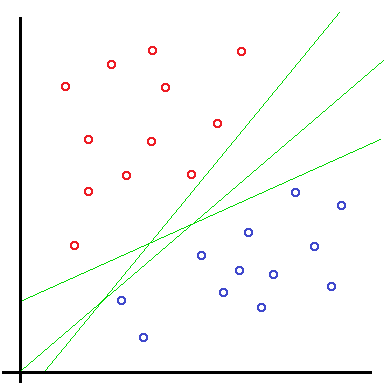
\includegraphics[width=5cm]{Img/Hyperplanes.PNG}
	\caption{Illustrates different hyperplanes to separate the classes}
	\label{fig:Hyperplanes}
\end{figure} 

If separating hyperplanes like these exist, it is possible to a very natural classifier, where a test observation is at assigned to a class depending on which side of the hyperplane its located. Then we classify the test observation based on the sign of $f(x^*) = \beta_0 + \beta_1 x_1^* + \beta_2 x_2^* + ... + \beta_p x_p^*$. If its positive then its assigned to class 1, and if its negative, then assigned to class -1. The magnitude of $f(x^*)$ tells us how far form the hyperplane the test variable is, which also tells us how certain we are about a class assignment. 

If there exist a hyperplane that perfectly separate out training data, that means there exist an infinite number of hyperplanes that perfectly separates the training data. And how to chose between this infinite number of hyperplanes to use as the classifier? This is where the Maximal Margin Classifier comes into the picture. This is selecting the hyperplane that is the farthest from the training data. This is done by calculating the perpendicular distance from each training observation.  The smallest distance from the training observation to the hyperplane is called the margin. \\
So, the aim is to generate a hyperplane that has the largest margin on the training set, and hop it also has a large margin on the test set. On \cref{fig:Hyperplane_margin} is illustrated the hyperplane using the Maximal Margin Classifier.

\begin{figure}[H]
	\centering
	\includegraphics[width=5cm]{Img/Hyperplane_margin.PNG}
	\caption{Hyperplane maximum margin}
	\label{fig:Hyperplane_margin}
\end{figure} 
The maximum hyperplane can be solved as follows: 
$$\underset{\beta_0 ,\beta_1 ,...,\beta_p}{\text{Maximize M}}$$

$$subject\: to\:\sum\limits_{j=1}^{p} \beta_j^2 = 1$$

$$y_i(\beta_0 + \beta_1 x_i1 + \beta_2 x_i2 + ... + \beta_p x_ip)  \geq  M\: \forall\: i=1,...,n$$
